\chapter{Architecture}
\section{Aperçu de l'architecture}

\begin{figure}[h]
  \label{fig:architecture}
  \center
  \setlength\fboxsep{5pt}
  \setlength\fboxrule{0.5pt}
  \fbox{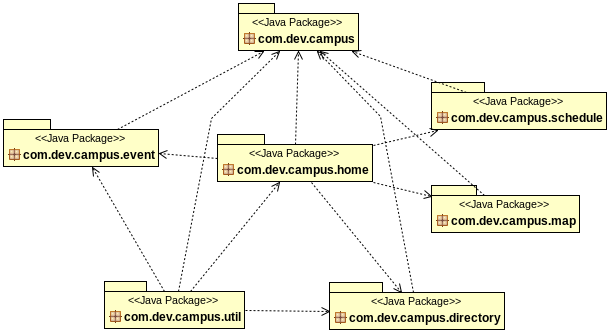
\includegraphics[width=0.9\textwidth]{resources/architecture.png}}
\end{figure}

L'application est organisée autour d'un ensemble d'activités Android, qui interagissent avec 4 modules différents. Ces modules sont organisés de la façon suivante: Settings, Directory, Events, et Analyser.

\newpage
\subsection{Settings}

\begin{figure}[h!]
  \label{fig:preferences_mod}
  \center
  \setlength\fboxsep{5pt}
  \setlength\fboxrule{0.5pt}
  \fbox{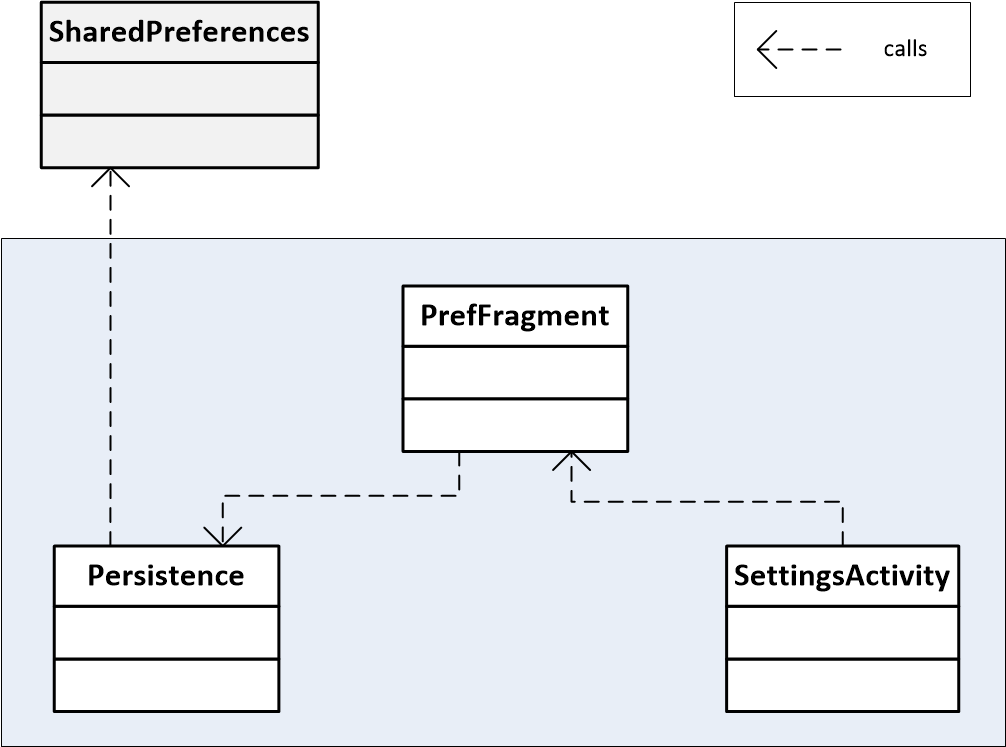
\includegraphics[width=0.5\textwidth]{resources/preferences_mod.png}}
\end{figure}

Ce module s'occupe de la gestion des préférences de l'utilisateur. Toutes les opérations de lecture/écriture des préférences sont effectuées à travers ce module, notamment la gestion des abonnements et des filtres.


\subsection{Directory}

\begin{figure}[h!]
  \label{fig:contacts_mod}
  \center
  \setlength\fboxsep{5pt}
  \setlength\fboxrule{0.5pt}
  \fbox{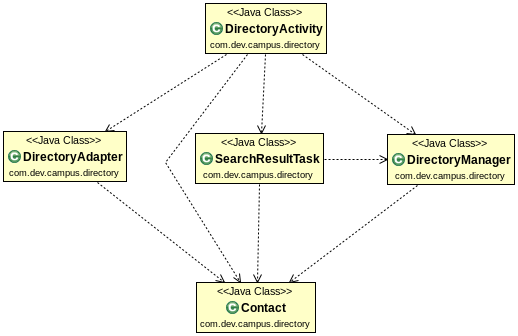
\includegraphics[width=0.4\textwidth]{resources/contacts_mod.png}}
\end{figure}

Ce module s'occupe de la gestion de l'annuaire. Il est responsable des services suivants:
\begin{itemize}
\renewcommand{\labelitemi}{$\bullet$}
\item Parsage des réponses LDAP / pages HTML.
\item Stockage et sauvegarde des données.
\item Affichage graphique des contacts de l'annuaire.
\end{itemize}

\subsection{Events}

\begin{figure}[h!]
  \label{fig:events_mod}
  \center
  \setlength\fboxsep{5pt}
  \setlength\fboxrule{0.5pt}
  \fbox{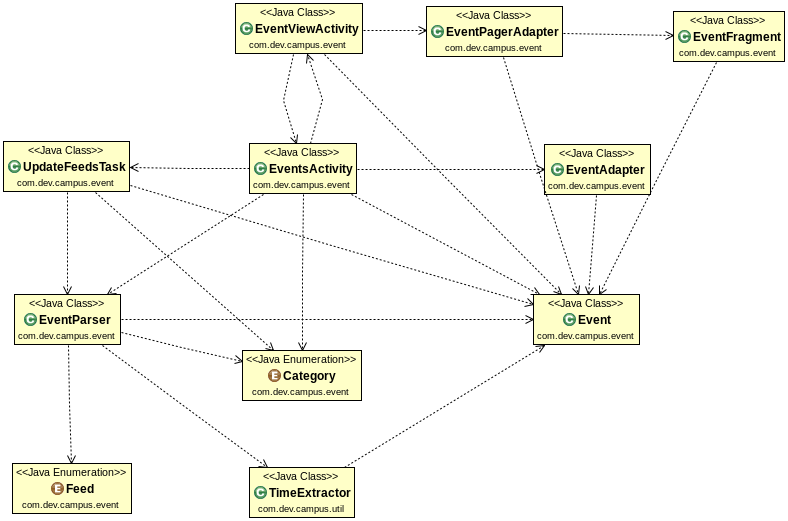
\includegraphics[width=0.65\textwidth]{resources/events_mod.png}}
\end{figure}

Ce module s'occupe de la gestion des événements. Il est responsable des services suivants:
\begin{itemize}
\renewcommand{\labelitemi}{$\bullet$}
\item Parsage des flux RSS / pages HTML.
\item Stockage et sauvegarde des données.
\item Affichage graphique des événements.
\end{itemize}


\subsection{Analyser}
Ce module s'occupe de l'analyse textuelle et de l'extraction d'information à partir d'un texte donné. On appelera ce module à travers l'interface de l'analyseur pour déterminer l'heure d'un événement donné (cf. figure~\ref{fig:events_mod}).